\documentclass[]{beamer}
% Class options include: notes, notesonly, handout, trans,
%                        hidesubsections, shadesubsections,
%                        inrow, blue, red, grey, brown

% Theme for beamer presentation.
\usepackage{beamerthemesplit} 
% Other themes include: beamerthemebars, beamerthemelined, 
%                       beamerthemetree, beamerthemetreebars  

\usetheme{Boadilla}
\setbeamertemplate{frametitle}[default][center]
\setbeamertemplate{footline}{\insertframenumber/\inserttotalframenumber}

\usepackage{amssymb}
\usepackage{amsmath}
\usepackage{ulem}
\setbeamertemplate{footline}[frame number]

\title{Lanczos Iteration Applied to the Variational Method in Quantum Mechanics} 
\author{Marcel Nunez}              
\institute{CHEG 827}     
\date{\today}                  

\begin{document}

% Creates title page of slide show using above information
\begin{frame}
  \titlepage
\end{frame}



\begin{frame}
  \frametitle{Quantum Mechanics} 

  \begin{itemize}
  \item<1-> Describes the behavior of small particles, such as electrons. Used to parameterize kinetic models in Catalysis research.
  \item<2-> Described by Schrodinger's Equation.
  \begin{equation*}
  \left( - \frac{\hbar ^2}{2m} \nabla ^2 + V(\textbf{r}) \right) \Psi (\textbf{r}) = E \Psi (\textbf{r})
  \end{equation*}
  \item<3-> In general, a difficult PDE to solve.
  \end{itemize}
  
\end{frame}



\begin{frame}
  \frametitle{Variational Approach}  

  \begin{itemize}
  \item<1-> Approximate the wavefunction as the sum of elements in an orthonormal basis set.
  \begin{equation*}
  \Psi(\textbf{r}) = c_1 \phi_1(\textbf{r}) +  c_2 \phi_2(\textbf{r}) + \cdots + c_N \phi_N(\textbf{r})
  \end{equation*}
  \item<2-> Maps $N$-dimensional vectors onto a subspace of possible wavefunctions.
  \item<3-> Orthonormality of basis vectors is desirable.
%  \begin{equation*}
%    < \phi_i | \phi_j> = \int_V \phi_i^*\phi_j dV = \delta_{ij}.
%    \end{equation*}
    
  \begin{equation*}
      \int_V \phi_i^*\phi_j dV = \delta_{ij}.
      \end{equation*}
    \end{itemize}
  
\end{frame}


\begin{frame}
  \frametitle{Matrix Representation of the Hamiltonian Operator}  
  
  \begin{itemize}
  \item<1-> Break the Hamiltonian into kinetic and potential contributions.
  \begin{equation*}
  \hat{H} = \hat{\mathrm{KE}} + \hat{\mathrm{PE}}
  \end{equation*}
  \item<2-> Define by how it operates on the basis wavefunctions.
  \begin{eqnarray*}
   \uuline{\hat{H}} = \begin{bmatrix}
        \int_V \phi_{1} ^* \hat{\mathrm{KE}} \phi_{1} dV &  \int_V \phi_{1} ^* \hat{\mathrm{KE}} \phi_{2} dV  & \ldots \\
            \int_V \phi_{2} ^* \hat{\mathrm{KE}} \phi_{1} dV  &  \int_V \phi_{2} ^* \hat{\mathrm{KE}} \phi_{2} dV & \ldots \\
            \vdots & \vdots & \ddots \\
        \end{bmatrix}\\+ \begin{bmatrix}
      \int_V \phi_{1} ^* \hat{\mathrm{PE}} \phi_{1} dV &  \int_V \phi_{1} ^* \hat{\mathrm{PE}} \phi_{2} dV  & \ldots \\
          \int_V \phi_{2} ^* \hat{\mathrm{PE}} \phi_{1} dV  &  \int_V \phi_{2} ^* \hat{\mathrm{PE}} \phi_{2} dV & \ldots \\
          \vdots & \vdots & \ddots \\
      \end{bmatrix}
  \end{eqnarray*}



  \end{itemize}
\end{frame}


 
\begin{frame}

 \frametitle{Plane-Wave Basis Set}
 
 \begin{columns}
   \begin{column}{0.4\textwidth}
     \begin{itemize}
         \item<1-> Exist for problems in a periodic box. 
         \item<2-> Kinetic energy can be computed analytically.
         \item<3-> Can compute potential part by using an FFT of the potential. 
     \end{itemize}
   \end{column}
 
   \begin{column}{0.6\textwidth}
      \begin{itemize}
         \item<1-> $\phi_{ijk}= \frac{1}{\sqrt{\Omega}} e^{iG_{ijk}\cdot r}$
         \item<2-> $\int_{V} \phi_{ijk}^* \left( -\frac{\hbar^2}{2m}\nabla ^2 \phi_{ijk}\right) dV = \frac{\hbar^2}{2m} |G_{ijk}|^2$
         \item<3-> $\hat{V}(r) = \sum_{ijk} \nu (i,j,k) e ^ {i G_{ijk} \cdot r}$
          \begin{eqnarray*}
          \frac{1}{\Omega} \int_V  \phi_{i+\Delta i,j+\Delta i,k+\Delta i} \hat{V}  \phi_{i,j,k} dV = \\ \nu(\Delta i,\Delta j, \Delta k)
          \end{eqnarray*}
      \end{itemize}
   \end{column}
 \end{columns}
 
  
\end{frame}




\begin{frame}
  \frametitle{Lanczos Algorithm}   

  \begin{itemize}
  \item<1-> Krylov method for quickly computing the few top magnitude eigenvalues.
  \begin{equation*}
  K_k (A,b) = \mathrm{span} \left\lbrace b,Ab,A^2 b,\cdots , A^{k-1}b \right\rbrace
  \end{equation*}
  \item<3-> Approximates a similarity transformation of the original matrix.
  \begin{equation*}
  A_k Q_k = Q_k T_k + B_k [0,\cdots , 0, q_{k-1}]
  \end{equation*}
  \item<4-> A slower method such as $QZ$ decomposition can compute the eigenvalues and eigenvectors of $T_k$.
  \end{itemize}
  
\end{frame}


\begin{frame}
  \frametitle{Test Case: 1-D Harmonic Oscillator}  

  \begin{itemize}
  \item<1-> $\hat{V}(x)=\frac{1}{2}m\omega^2x^2$
  \item<2-> One of the few quantum problems for which an analytical solution exists.
  \begin{eqnarray*}
  \Psi_n(x) &&= \frac{1}{\sqrt{2^m n!}} \left( \frac{m \omega}{\pi \hbar} \right)^{\frac{1}{4}} e^{ -\frac{m\omega x^2}{2\hbar} }H_n \left( \sqrt{\frac{m \omega}{\hbar}}x \right)\\
  E_n &&= \hbar \omega (n+\frac{1}{2})
  \end{eqnarray*}
  \end{itemize}
  
\end{frame}



\begin{frame}
  \frametitle{Accuracy}  

  \begin{columns}
  
  \begin{column}{0.5\textwidth}
  \centering
  
  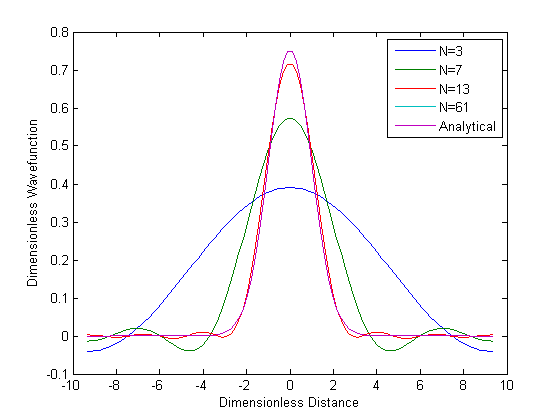
\includegraphics[height=1.2in]{a1.png}
    
  Numerical and analytical solutions

  \pause
  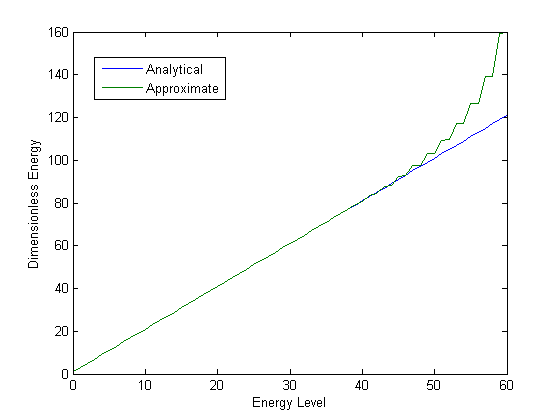
\includegraphics[height=1.2in]{a2.png}
  
  Numerical and analytical energies.

  \end{column}
  
  \begin{column}{0.5\textwidth}
  \centering
  
  \pause
  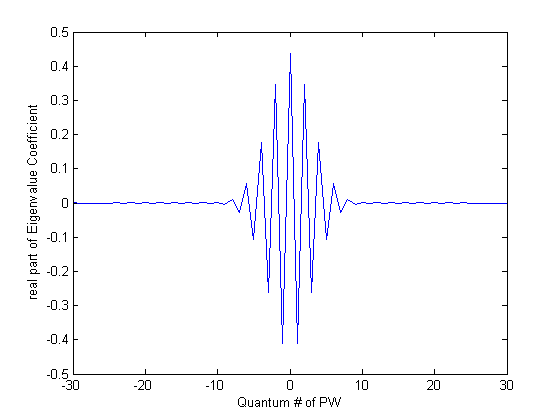
\includegraphics[height=1.2in]{a3.png}
  
  Plane-wave coefficients.
    
  \pause  
  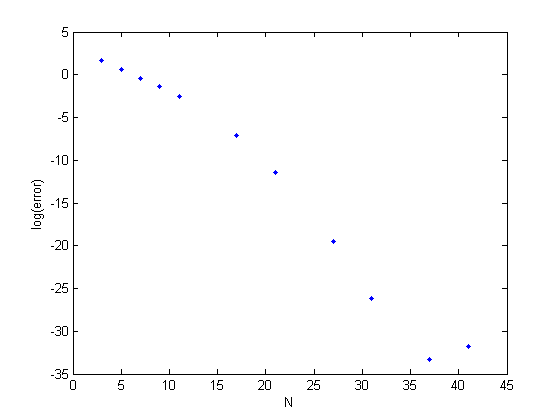
\includegraphics[height=1.2in]{a4.png}
  
  Error behavior.
  \end{column}
  
  \end{columns}
  
\end{frame}


\begin{frame}
  \frametitle{Speed}  

  \begin{columns}
    
    \begin{column}{0.5\textwidth}
    \centering
    
    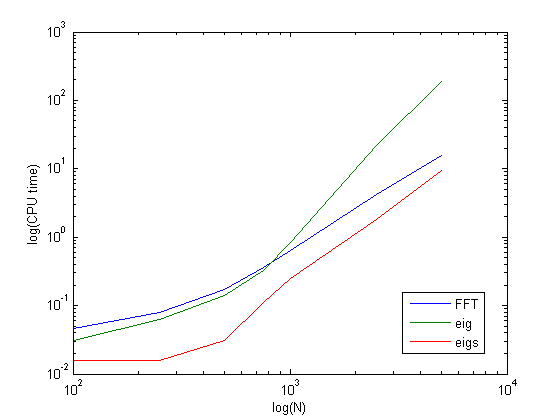
\includegraphics[height=1.8in]{s1.png}
      
    Speed of various parts of the calculation.
  
    \end{column}
    
    \begin{column}{0.5\textwidth}
    \centering
      
    \pause  
    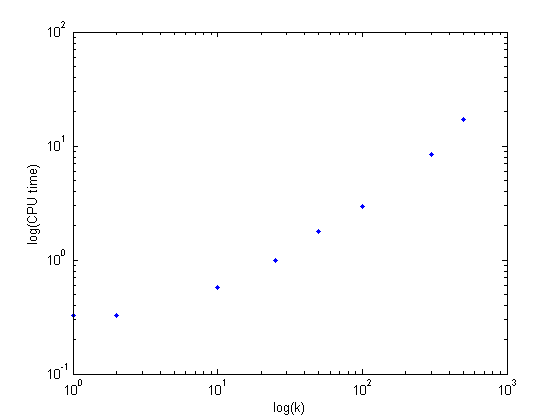
\includegraphics[height=1.8in]{s2.png}
    
    Speed of Lanczos vs. k.
    \end{column}
    
    \end{columns}
  
\end{frame}


\begin{frame}
  \frametitle{Conclusions}  

  \begin{itemize}
  \item<1-> Finding eigenvalues and eigenvectors is limiting in speed of the calculation.
  \item<2-> The Lanczos Algorithm can quickly compute the smallest eigenvalues, which are the ones well represented by the variational approach.
  \item<3-> Only about 60 basis functions are needed for the case studied, but this will change in higher dimensions.
  \end{itemize}
  
\end{frame}



%\begin{frame}
%  \frametitle{Matrix Representation of the Hamiltonian Operator}   % Insert frame title between curly braces
%  
%  \begin{columns}[c]
%  \column{2in}  % slides are 3in high by 5in wide
%  \begin{itemize}
%  \item<1-> First item
%  \item<2-> Second item
%  \item<3-> ...
%  \end{itemize}
%  
%  \column{2in}
%  \framebox{Insert graphic here % e.g. \includegraphics[height=2.65in]{graphic}
%  }
%  \end{columns}
%  
%\end{frame}


\end{document}
